\section*{Problem 5:}
\paragraph{System Specs:} All our experiments run on Intel(R) Xeon(R) CPU E3-1280 v5 with 3.70 GHz and 32 GB of RAM on 64-bit operating system running Windows 7. 

\paragraph{Code:} We provide a single file \texttt{driver.m} that generates all the data in the tables and plots by running it. It calls the necessary function and load the examples one after another. 
 
\paragraph{Plots:} Figure~\ref{fig:all} shows the results of the three algorithms plotted on top of each others. It shows that Lanczos-based algorithm is able to capture $Z(s)$ almost exactly using $k=100$. For such value of $k$, the textbook algorithm will return NaN everywhere. Thus, we used $k=10$ in the plot. Function \texttt{Figure\_1()} in \texttt{driver.m} file generates this plot. 

\begin{figure}[!tbh]
\centering        
   \subfloat {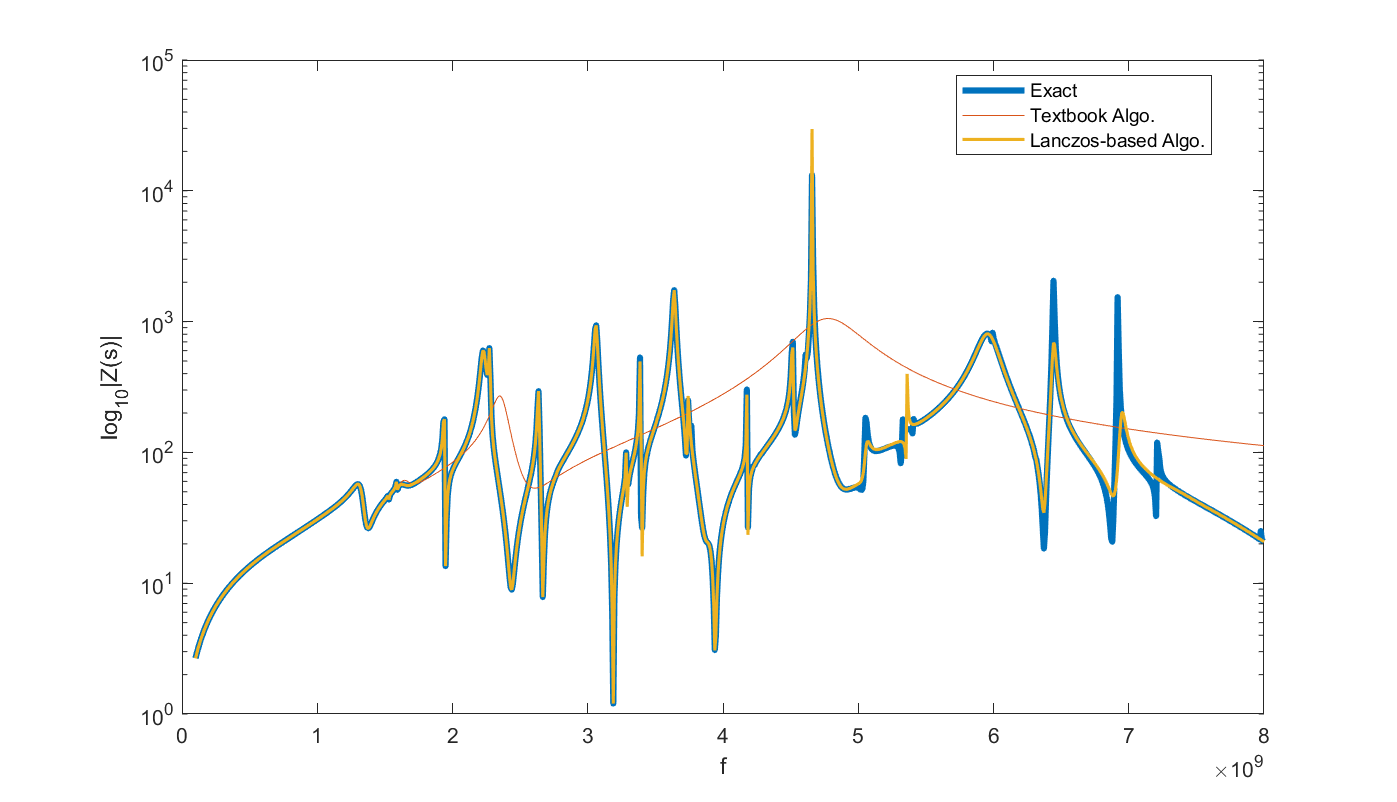
\includegraphics[width=0.85\textwidth]{../code/figure1.png}}
   \caption{The results of the three algorithms; exact algorithm, textbook algorithm with $k=10$, and Lanczos-based algorithm with $k=100$. We used expansion point $s_{0} = \expnumber{1}{5} + 2\pi i \expnumber{5.5}{8}$ for both algorithms.   }
   \label{fig:all}
\end{figure}

\paragraph{$s_0$ with fast convergence:} We test our implementation of the textbook and Lanczos-based algorithm for different values of $s_{0}$ and found that it runs fairly fast for the small input given in \texttt{FP\_Ex1.mat}; it takes less than a second even for large i.e., $k < 100$. 

We followed the recommendation given in the lectures for how to pick $s_{0}$. We choose $s_{0} = \expnumber{1}{5} + 2\pi i \expnumber{5.5}{8} $. 

\paragraph{Comparison:} We run both our implementation for different values of $k$ and the above $s_{0}$ and compared between both. Table~\ref{tab:comp} shows the average different ($\parallel \cdot \parallel^{2}$) and the maximum (absolute) different between the two vectors containing the output of both algorithms for different values of $s$. Function \texttt{Table\_1()} in \texttt{driver.m} file generates these data. We can see that when $k>13$, the two algorithms will give difference numerical results. 

\begin{table}[!tbh]
 \centering    
\begin{tabular}{ ||p{1.5cm}| p{4cm}| p{4cm}||}
\hline
 $k$  & Average Difference & Maximum Difference \\ \hhline{|=|=|=|}   
    2   & $\expnumber{2.082747}{-28}$   & $\expnumber{2.109424}{-15}$   \\
	3   & $\expnumber{7.919421}{-27}$   & $\expnumber{6.439294}{-15}$   \\
	4   & $\expnumber{5.026520}{-25}$   & $\expnumber{4.618528}{-14}$   \\
	5   & $\expnumber{8.547583}{-26}$   & $\expnumber{2.664535}{-14}$   \\
	6   & $\expnumber{3.052289}{-23}$   & $\expnumber{4.112266}{-13}$   \\
	7   & $\expnumber{1.148403}{-19}$   & $\expnumber{4.235057}{-11}$   \\
	8   & $\expnumber{2.656897}{-17}$   & $\expnumber{3.190033}{-09}$   \\
	9   & $\expnumber{6.690131}{-15}$   & $\expnumber{1.812676}{-08}$   \\
	10  & $\expnumber{6.292776}{-12}$   & $\expnumber{3.008865}{-07}$   \\
	11  & $\expnumber{7.619719}{-11}$   & $\expnumber{6.315981}{-06}$   \\
	12  & $\expnumber{4.360106}{-04}$   & $\expnumber{1.650155}{-02}$   \\
	13  & $\expnumber{9.107709}{-04}$   & $\expnumber{1.494378}{-02}$   \\
	14  & $\expnumber{7.052574}{+00}$   & $\expnumber{3.945073}{-01}$   \\
	15  & $\expnumber{5.904627}{+01}$   & $\expnumber{1.279984}{+00}$   \\
	16  & $\expnumber{1.779754}{+02}$   & $\expnumber{1.488481}{+00}$   \\
	17  & $\expnumber{1.105689}{+02}$   & $\expnumber{1.625567}{+00}$   \\
	18  & $\expnumber{1.100795}{+02}$   & $\expnumber{1.632208}{+00}$   \\
	19  & $\expnumber{1.219843}{+02}$   & $\expnumber{1.688382}{+00}$   \\
	20  & $\expnumber{1.075413}{+02}$   & $\expnumber{9.725151}{-01}$   \\
	21  & $\expnumber{1.108709}{+02}$   & $\expnumber{1.217680}{+00}$   \\
	22  & $\expnumber{4.712087}{+02}$   & $\expnumber{1.762950}{+00}$   \\
	23  & $\expnumber{1.160591}{+03}$   & $\expnumber{2.593543}{+00}$   \\
	24  & $\expnumber{3.507356}{+03}$   & $\expnumber{4.102138}{+00}$   \\
	25  & $\expnumber{7.329648}{+03}$   & $\expnumber{5.568756}{+00}$   \\
	26  & $\expnumber{2.245490}{+04}$   & $\expnumber{8.889336}{+00}$   \\
	27  & $\expnumber{2.633420}{+04}$   & $\expnumber{9.681861}{+00}$   \\
	28  & $\expnumber{4.881768}{+04}$   & $\expnumber{1.252447}{+01}$   \\
	29  & $\expnumber{7.066637}{+04}$   & $\expnumber{1.471937}{+01}$   \\
	30  & $\expnumber{1.151561}{+05}$   & $\expnumber{1.801101}{+01}$   \\
\hline
\end{tabular} 
\caption{Average and maximum (absolute) difference between the results of the textbook algorithm and Lanczos approach for different $k$ values.}
   \label{tab:comp}
\end{table}

\paragraph{Explanation:} We believe the reason why the textbook algorithm does not perform well is because it depends on computing $M^{j}r$ (to compute the moments) for increasing values of $j$ which convergences quickly to the the eigenvector of $M$ with largest eigenvalue. Thus, the information it contains comes from a single eigenvector where the information should comes from all eigenvectors of $M$. In contrast, Lanczos's $T_{k}$ represents oblique projection of $M$ onto the $K_{k}(M,r)$ Krylov subspace which contains information about $k$ eigenvectors. 

\paragraph{Lanczos approach with difference $s_{0}$:} For this experiment, we defined the ``good approximation'' such that the average difference between the Lanczos-based algorithm and the exact algorithm is less than  $10^{-5}$. We tested using different $s_{0}$ and for each value we run the algorithm in a loop for $200\leq k \leq 1000$ and stop when the results meet the good-approximation criterion we set thus obtaining the minimum $k$ value that results into the best approximation given $s_{0}$. Table~\ref{tab:s0} show the results for different $s_{0}$. Function \texttt{Table\_2()} in \texttt{driver.m} file generates these data.

We notice that complex $s_{0}$ take more time for the same $k$ value (first and last row in Table~\ref{tab:s0}. Expansion point with complex part equal to the maximum or minimum frequency take double the time it takes for $s_{0}$ suggested in the lecture notes. Getting closer y-axis can results in higher $k$ values and thus slower convergence. 


\begin{table}[!tbh]
 \centering    
\begin{tabular}{ ||p{3.0cm}|p{1.5cm}| p{4cm}| p{4cm}||}
\hline
 $s_{0}$  & $k$ & Time & Average Difference \\ \hhline{|=|=|=|=|}   
 $10^{5} + 2 \pi i f_{avg}$  & 212 & 3.416422 & $\expnumber{7.9513}{-6}$\\
 $10^{5} + 2 \pi i f_{min}$ & 278 & 7.300847 & $\expnumber{6.419988}{-6}$\\
 $10^{5} + 2 \pi i f_{max}$ & 262 & 6.130839 & $\expnumber{8.102979}{-7}$ \\
 $10^{9} $                  & 290 & 6.739243 & $\expnumber{8.396701}{-6}$ \\
 $10^{10}$                  & 212 & 2.901619 & $\expnumber{4.187281}{-6}$  \\  
\hline
\end{tabular} 
\caption{Lanczos approach using different $k$ and $s_{0}$ values and comparing it with the exact solution ($f_{avg} = \frac{f_{min}+f_{max}}{2}$) }
   \label{tab:s0}
\end{table}